\documentclass[../manuale_utente.tex]{subfiles}
\begin{document}


\subsection{Creazione workflow}
    \label{sub:crea_work}
\subsubsection{Caricamento dati}
    \label{subsub:carica_dati}

Il primo passo per poter utilizzare HD-Viz è importare dei dati. È possibile farlo in due modi:
\begin{itemize}
    \item caricamento di dati tramite file \glossario{CSV} da locale
    \item caricamento di dati tramite query da un database esterno
\end{itemize}
In seguito l’utente potrà esplorare e manipolare i grafici al fine di analizzare i dati, trarne conclusioni e similitudini tra essi. \\
Per importare un file da locale è sufficiente andare nella sezione \emph{“Carica file”}  in alto a sinistra, cliccare su \emph{“scegli file”}, scegliere un file CSV presente sul proprio dispositivo e poi cliccare su \emph{“Carica”}. 
Per importare dati tramite database bisogna cliccare sul bottone \emph{“Carica”} presente nel riquadro in alto a sinistra, relativo al caricamento database.
In questo modo il database verrà caricato tramite un file di configurazione presente nella cartella  \verb|server/src/dbConfig|

\begin{figure}[H]
	\centering
	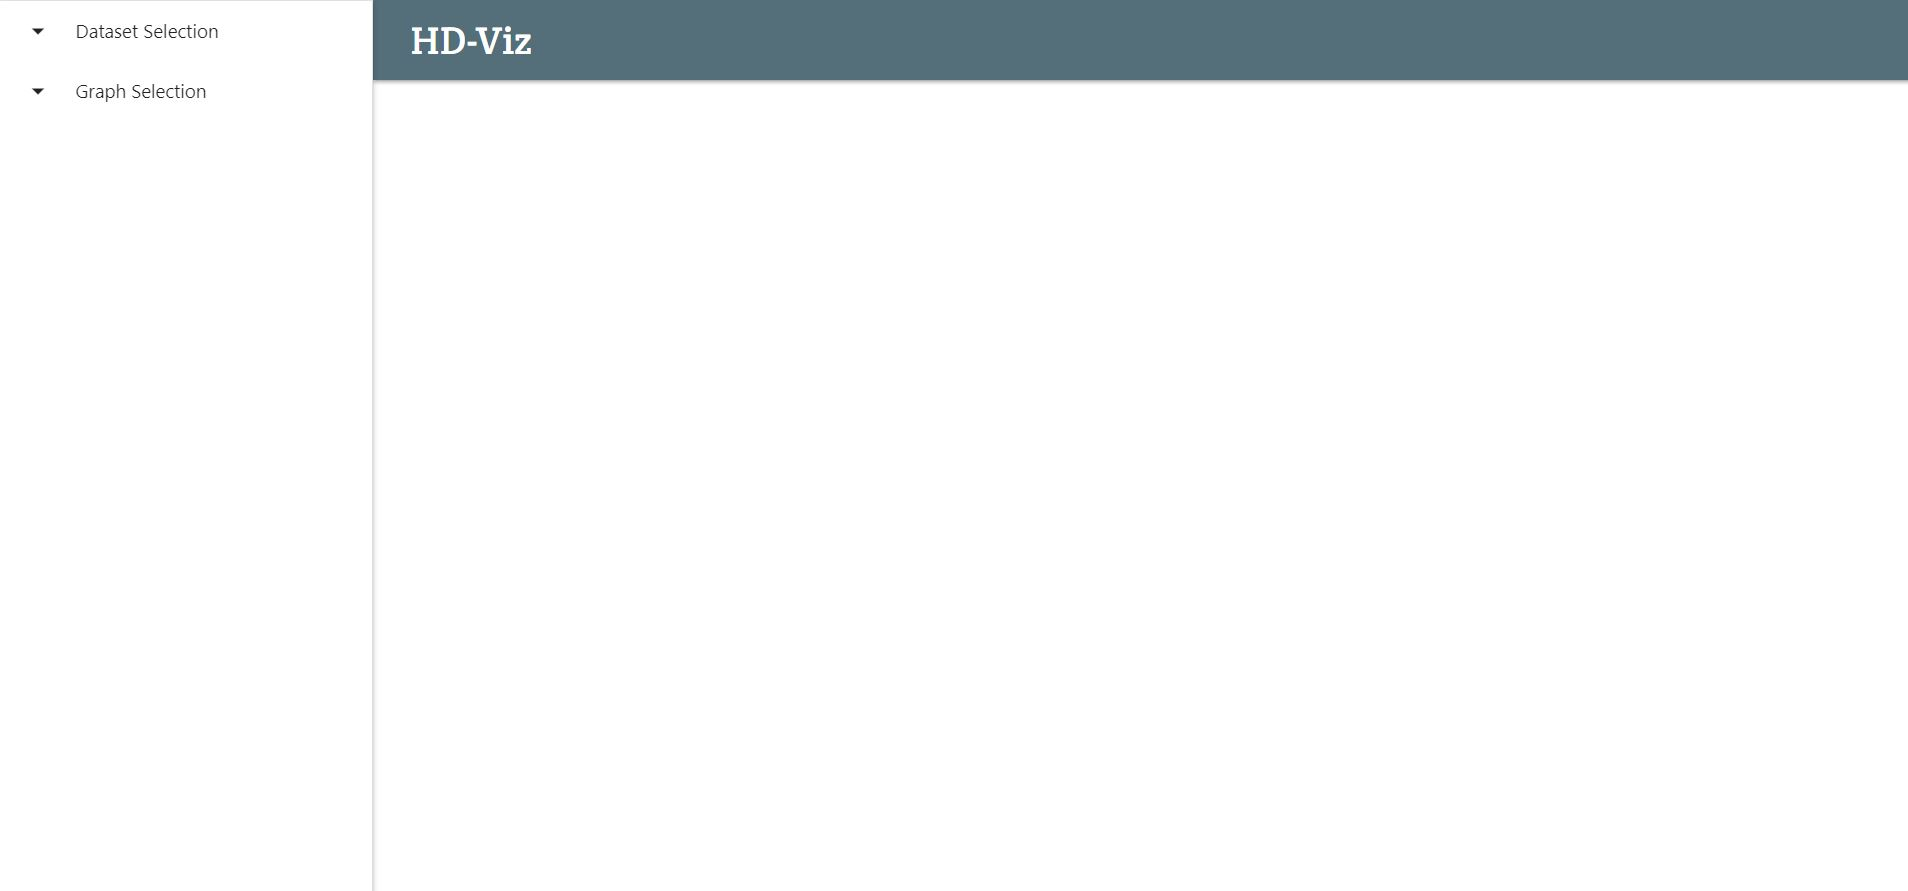
\includegraphics[width=18cm]{src/img/introduzione.jpg}
	\caption{Introduzione a Hd-Viz}
\end{figure}

\begin{figure}[H]
	\centering
	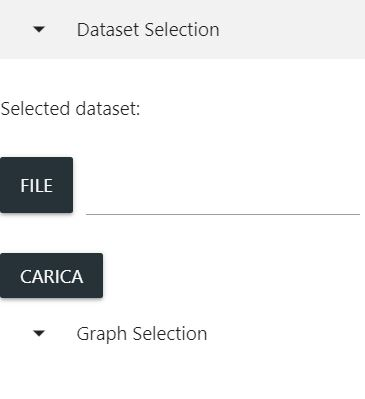
\includegraphics[width=18cm]{src/img/seleziona_dataset.jpg}
	\caption{Seleziona fonte}
\end{figure}

\subsubsection{Visualizzazione grafico}
    \label{subsub:vis_graf}
Una volta che il file è stato caricato, il grafico principale, lo \glossario{ScatterPlot Matrix}, verrà definito con i dati appena passati. \\
Grazie al menu a tendina in alto a sinistra sarà possibile cambiare grafico passando per esempio al Force Field, all’Heat Map etc.

\paragraph{ScatterPlot Matrix}
    \label{par:vis_scatt}
Si tratta di un grafico che permette di visualizzare la relazione tra due variabili quantitative riportate su uno spazio cartesiano. Ogni unità statistica è rappresentata da un punto posizionato sul grafico in base alle sue coordinate. 
Quindi questo grafico sarà costituito da tanti punti quante sono le unità statistiche oggetto di studio. I valori che assume l’unità statistica per le due variabili rappresentano quindi la posizione dell’unità rispetto agli assi. 
Osservando l’andamento dei punti si può notare come sembra esserci una relazione lineare positiva o negativa. Se il modello di punti sul grafico scende dall'alto a sinistra verso il basso a destra, suggerisce una correlazione negativa. 
Può essere disegnata una linea di andamento (o linea di trend) per studiare la correlazione tra le variabili in esame. Se non c’è relazione tra le due variabili all’aumentare dei valori di una variabile, i valori dell’altra variabile non risulteranno in media né aumentare né diminuire.\\
In questo grafico sarà possibile modificare la dimensione del dataset, la dimensione della matrice, modificarne la dimensione rappresentata mediante tinta, mediante brillanza. Tutti questi parametri si troveranno
in ordine in un menu a sinistra. Ad ogni manipolazione dei parametri inseriti si otterrà subito una modifica del grafico. \\
Qui di seguito per esempio ecco come si mostra uno ScatterPlot Matrix al caricamento dei dati dell'Iris.

\begin{figure}[H]
	\centering
	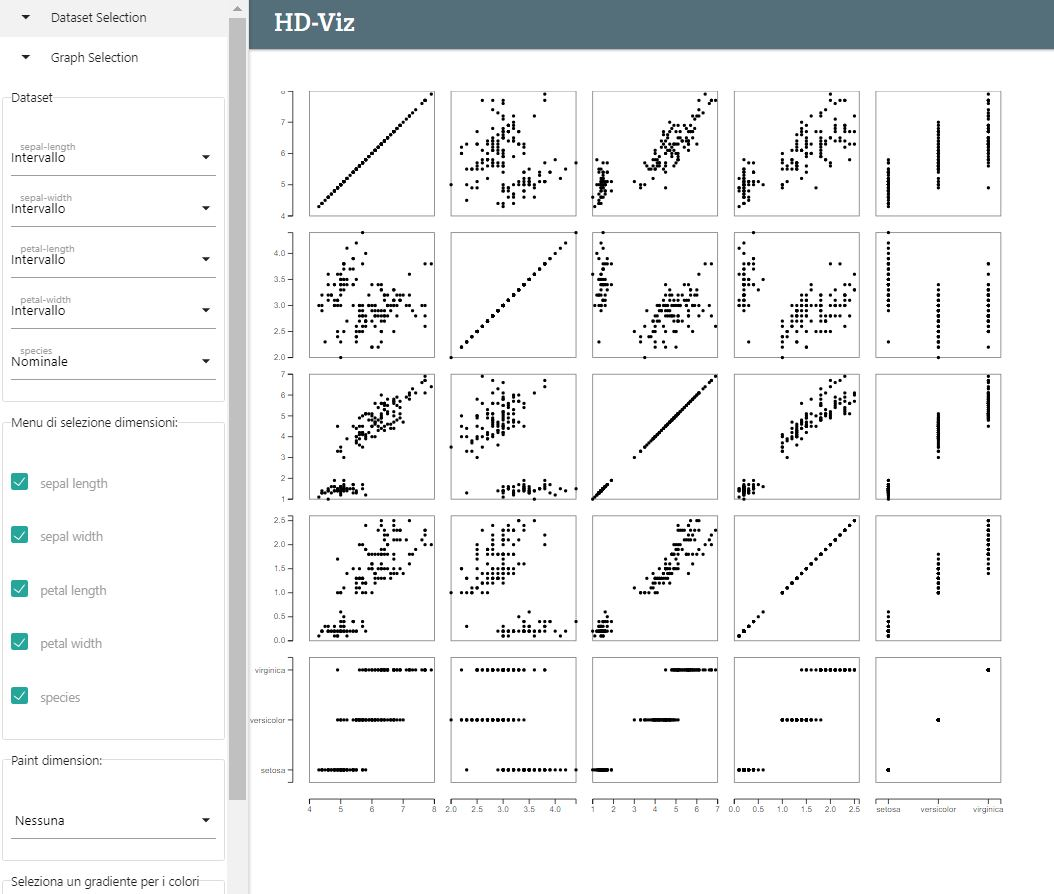
\includegraphics[width=18cm]{src/img/spm/spm_iris.jpg}
	\caption{ScatterPlot Matrix iris dataset}
\end{figure}

Quando si va a dare colore alla lunghezza dei sepali, il risultato è il seguente:

\begin{figure}[H]
	\centering
	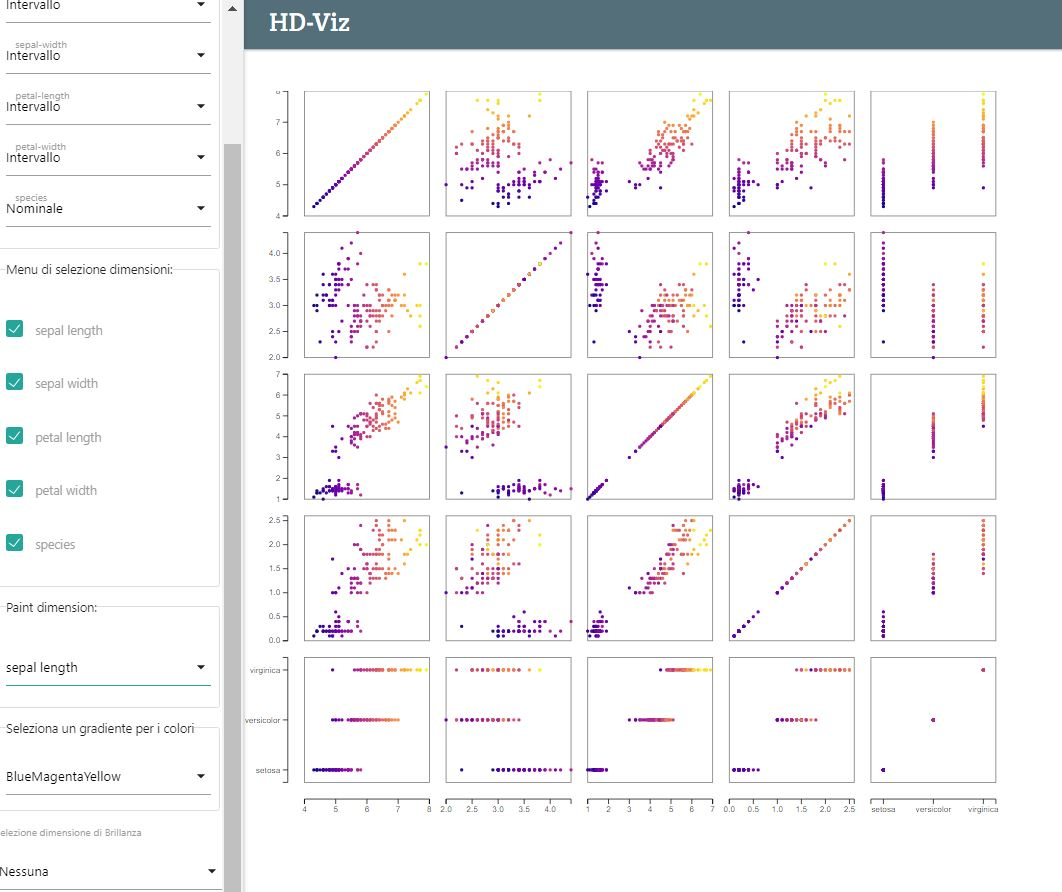
\includegraphics[width=18cm]{src/img/spm/spm_colore_dimensione_sepal.jpg}
	\caption{ScatterPlot Matrix lunghezza del sepalo colorato}
\end{figure}

È possibile inoltre cambiare i colori rappresentati. Nel seguente esempio si è scelto di colorare la dimensione del sepalo, e si è usato come gradiete il CoolWarm.

\begin{figure}[H]
	\centering
	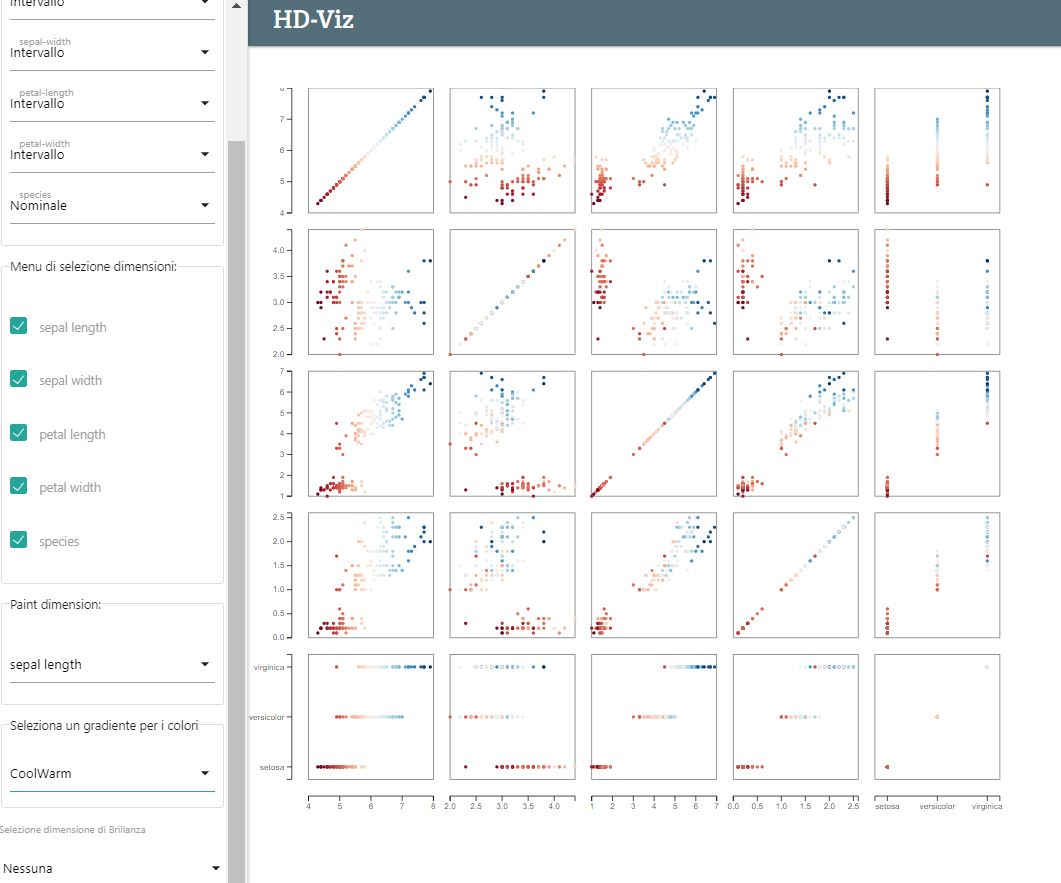
\includegraphics[width=18cm]{src/img/spm/spm_mix_colori.jpg}
	\caption{ScatterPlot Matrix modifica di più colori}
\end{figure}


Qui invece vi è un esempio con un \glossario{dataset} da 1000 records. È possibile cambiare le dimensioni rappresentate escludendone una ed aggiungendone un'altra, come rappresentato in figura.

\begin{figure}[H]
	\centering
	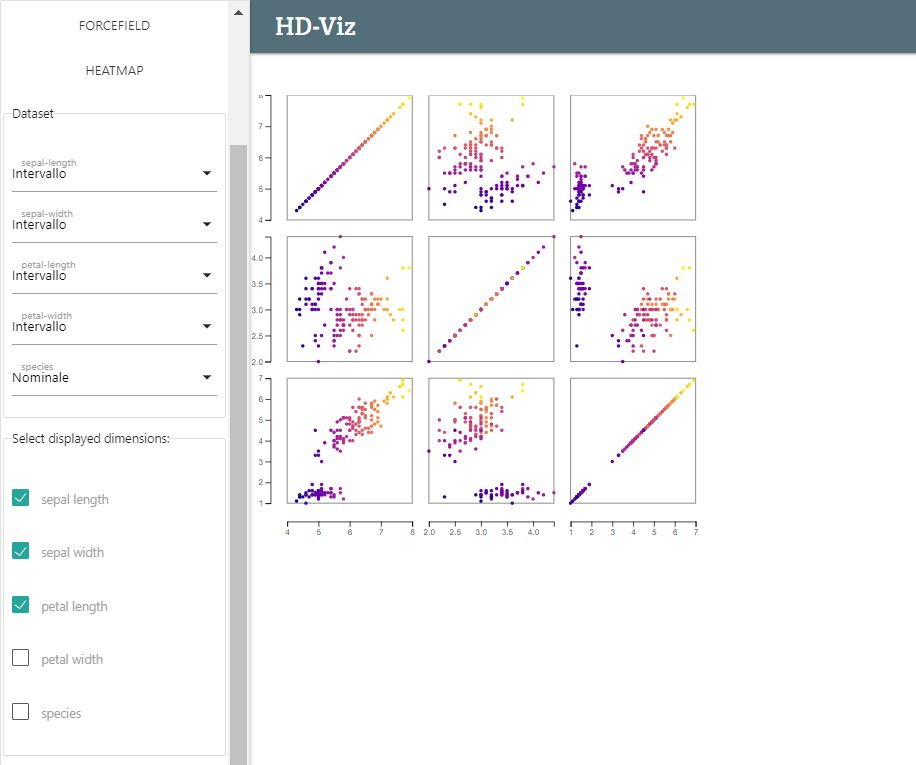
\includegraphics[width=18cm]{src/img/spm/spm_cambio_dim.jpg}
	\caption{ScatterPlot Matrix modifica delle dimensioni rappresentate}
\end{figure}


%
%\subsection{Modifica workflow}
%    \label{sub:mod_work}
%\subsubsection{Modifica dati}
%    \label{subsub:mod_dati}
%
%HD-Viz offre la possibilità di manipolare i grafici forniti, intervenendo sulle dimensioni tramite un pannello di controllo presente alla sinistra di ogni grafico. 
%Tra le varie modifiche che è possibile fare vi è la possibilità di: 
%\begin{itemize}
%	\item \emph{modificare la dimensione del dataset corrente};
%	\item \emph{modificare la dimensione della matrice per lo ScatterPlot Matrix};
%	\item \emph{modificare la dimensione rappresentata mediante tinta per lo ScatterPlot Matrix};
%	\item \emph{modificare la dimensione rappresentata mediante brillanza per lo ScatterPlot Matrix};
%	\item \emph{modificare la distanza nel grafico DistanceMap, ForceField};
%	\item \emph{modificare il preprocessing dei dati nel grafico DistanceMap, ForceField};
%	\item \emph{modificare l’influenza di una dimensione nel grafico DistanceMap, ForceField};
%	\item \emph{modificare la posizione dei nodi nel grafico ForceField};
%	\item \emph{rimuovere degli archi nel grafico ForceField};
%	\item \emph{modificare la scala della forza nel grafico ForceField};
%	\item \emph{modificare il gradiente di colori nel grafico DistanceMap};
%	\item \emph{modificare l’ordinamento nel grafico DistanceMap};
%	\item \emph{modificare le etichette nel grafico DistanceMap};
%
%	\item \emph{modificare il gradiente di colori nel grafico HeatMap};
%	\item \emph{modificare le etichette nel grafico HeatMap};
%	\item \emph{modificare l’ordinamento nel grafico HeatMap}.
%\end{itemize}


\end{document}